\documentclass[11pt,a4paper,oneside]{article}
\usepackage[latin1]{inputenc}
\usepackage{amsmath}
\usepackage{amsfonts}
\usepackage{amssymb}
\usepackage{graphicx}
\usepackage{color}
\usepackage {tikz}
\usepackage{fancyvrb}
\usetikzlibrary {er}
\usepackage[left=2.00cm, right=2.00cm, top=1.00cm]{geometry}
\graphicspath{{./}}
\fvset{tabsize=4}

\begin{document}
	\title{DS 221 - Introduction to Scalable Systems \\ Parallelization of KMeans Clustering using OpenMP}
	\author{Shriram R. \\ M Tech (CDS) \\ 06-02-01-10-51-18-1-15763}
	\maketitle
	
	\section{Introduction}
	KMeans Clustering algorithm has been parallelized using OpenMP and the speedup for different thread counts and schedule configurations were observed through experiments. The following sections cover the methodology, experimental setup and results in detail.
	
	\section{Methodology}
	The algorithm runs for a fixed number of iterations (currently 100) for convergence of centroids. This stopping criteria is to enable consistent comparison. The following steps are followed in each iteration:
	\begin{enumerate}
		\item A parallel region with given no. of threads is started with the points, centroid, label and temp array in shared mode. The temp array is used to store updated centroid info for each thread:
		\begin{enumerate}
		\item The set of points is distributed among the threads using either static or dynamic chunks.
		\item Each thread will assign its points to their nearest centroid by computing the euclidean distance and updates the corresponding entry in the label array
		\item Each thread also updates the temp array with its local cluster size and centroid values
	    \end{enumerate}
		\item Global centroid information is updated by aggregating the thread level centroids computed in the previous step and is used for the next iteration. This is a sequential step
	\end{enumerate}
    The above methodology is illustrated in the code snippet in the appendix.
	
	
	\section{Experimental Setup}
	Experiments were run on a single compute node having 8 core AMD Opteron 3380 processor and 32GB RAM in the Turing compute cluster. Batch job was created using a shell script and executed through PBS. For each thread count, two experiments, one with static and other with dynamic chunk sizes were performed.\\
	\newline
	The time taken to run the KMeans clustering was measured using C library functions and was printed to stdout along with specified output. Each experiment was repeated 20 times consecutively and then the average was computed for the plots and analysis. \\
	\newline
	In each experiment, both sequential and parallel versions of code were executed so as to remove bias from other system load. The time measured is only for the algorithm and therefore excludes any input read and output writes in the program.\\
	\newline
	
	\begin{verbatim}
					
							
	\end{verbatim}
	
	\section{Results}
	
	The experimental results for large dataset (500000 points) are tablulated and plotted below,
	
	  \begin{center}
		\begin{tabular}{|l|c|c|c|c|}
			\hline 
			\textbf{Schedule} & \textbf{Threads}  & \textbf{Sequential (Avg.) (s)} & \textbf{Parallel (Avg.) (s)} & \textbf{Speedup} \\
			\hline
		    Static & 4 &  8.077 & 4.378 & 1.845\\ 
			\hline 
		     Static & 8 &  8.053 & 3.159 & 2.549\\
			\hline 
			 Static & 16 &  8.086 & 3.294 & 2.454\\
			\hline 
			 Dynamic & 4 &  8.079 & 4.259 & 1.896\\ 
			\hline 
			Dynamic & 8 &  8.053 & 2.780 & 2.896 \\
			\hline 
			Dynamic & 16 &  8.041 & 2.911 & 2.763\\
			\hline 
		\end{tabular}
	\end{center}
	
	\begin{center}
		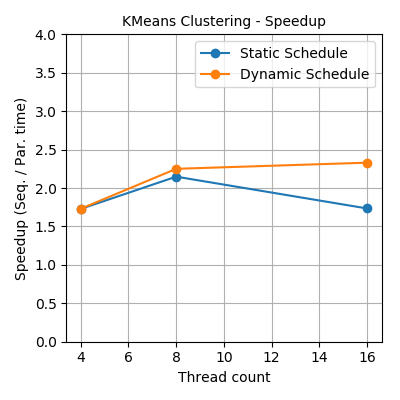
\includegraphics[scale=0.6]{1.png}		
	\end{center}

    \begin{center}
    	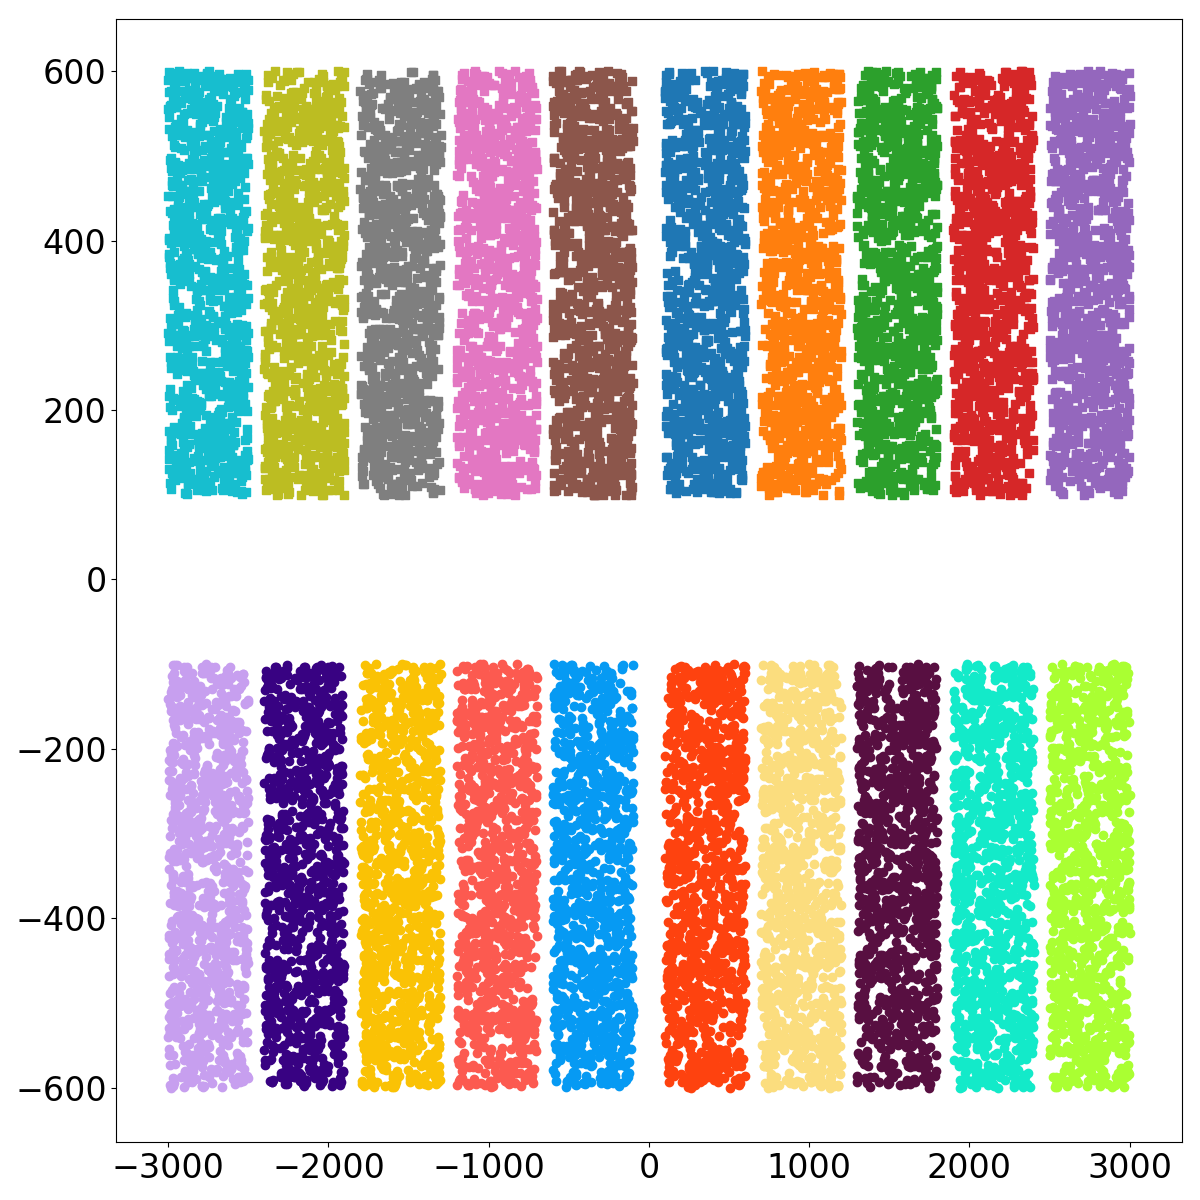
\includegraphics[scale=0.2]{2.png}	\\
    	Clusters Formed by KMeans Algorithm for 500000 points
    \end{center}
	 
	\begin{verbatim}
	 
	 
	\end{verbatim}
     
    \section{Observations}
    It can be observed that the speedup increases with number of threads upto 8 and then decreases in the case of static scheduling. This is because a single node can run only maximum of 8 threads in parallel. Any additional increase in the thread count would result in more context switches thereby reducing the speedup. \\
    \newline
    In the dynamic scheduling, the speedup increases even for 16 threads since the iterations from waiting threads can be distributed to the threads in execution thereby the computation does not have to wait for CPU to be available. It can be observed that dynamic scheduling was more efficient than static.  \\
    \newline
    The speedup is less than the thread count as the program contains both serial and parallel regions. In addition, there is a overhead of creating and managing threads in each iteration which reduces the speedup further.     
    
    \section{References}
    \begin{list}{}{}
    	\item 1. https://en.cppreference.com/w/c
    	\item 2. DS 221 Course lecture notes
    	\item 3. https://computing.llnl.gov/tutorials/openMP/
    	\item 4. http://www.arc.ox.ac.uk/content/pbs-job-scheduler
    	\item 5. https://www.dartmouth.edu/~rc/classes/intro\_openmp/print\_pages.shtml
    \end{list}

    \section{Appendix - Code} 
    
    \begin{Verbatim}
    for (int i = 0; i < ITER; i++)
    {	
    	// Parallel region
    	#pragma omp parallel num_threads(THREADS) shared(pts, label, centroid, temp)
    	{	
    		float min_dist, dist;
		    int tid, min_label;
		    tid = omp_get_thread_num();
    
		    // Reset temp
		    for (int k = 0; k < CLUSTERS; k++)
		    {
			    temp[tid][k][0] = 0;
			    temp[tid][k][1] = 0;
			    temp[tid][k][2] = 0;
		    }
		    
		    
		    
		    
    
		    // Assign Labels for all points
		    #pragma omp for schedule(static, CHUNKSIZE)
		    for (int j = 0; j < SIZE; j++)
		    {
			    min_dist = FLT_MAX;                
			    for (int k = 0; k < CLUSTERS; k++)
			    {
				    dist = (pts[j][0] - centroid[k][0]) * (pts[j][0] - centroid[k][0]) +
				    (pts[j][1] - centroid[k][1]) * (pts[j][1] - centroid[k][1]);
				    if (dist < min_dist)
				    {
					    min_dist = dist;
					    min_label = k;
			    	}
		    	}
			    label[j] = min_label;
			    temp[tid][min_label][0] += pts[j][0];
			    temp[tid][min_label][1] += pts[j][1];
			    temp[tid][min_label][2] += 1; 
    		}
    	}
	    // End of parallel region
	    
	    // Collect temp
	    for (int j = 1; j < THREADS; j++)
	    {
		    for (int k = 0; k < CLUSTERS; k++)
		    {
			    temp[0][k][0] += temp[j][k][0];
			    temp[0][k][1] += temp[j][k][1];
			    temp[0][k][2] += temp[j][k][2];
		    }
	    }
    
	    // Compute and update centroid
	    for (int k = 0; k < CLUSTERS; k++)
	    {
		    if (temp[0][k][2] == 0)
		    	continue;
		    centroid[k][0] = temp[0][k][0] / temp[0][k][2];
		    centroid[k][1] = temp[0][k][1] / temp[0][k][2];
	    }
    }
    \end{Verbatim}
    
    \begin{center}
    	-----------End of Report------------
    \end{center}
    
\end{document}